\themaM
\graphicspath{{../Ch22_Les_angles/Images/}}

\chapter{Mesurer et\\représenter\\un angle}
\label{C28}


%%%%%%%%%%%%%%%%%%%%%%%%%%%%%%%%%%%%%%%%%
%%%%%%%%%%%%%%%%%%%%%%%%%%%%%%%%%%%%%%%%%
\begin{prerequis}[Connaissances et compétences associées]
   \begin{itemize}
      \item Utiliser le rapporteur pour déterminer la mesure en degré d’un angle ; construire un angle de mesure donnée en degrés.
      \item Lire ou construire des représentations de données : diagrammes circulaires ou semi-circulaires.
   \end{itemize}
\end{prerequis}

\vfill

\begin{debat}[Débat : degré et rapporteur]
   Le {\bf degré} (comme mesure d'angle, pas de température !) vient des babyloniens, qui comptaient en base sexagésimale (60). Il correspond à 1/360 d'un tour complet. L'origine de 360 n'est pas établie avec certitude, mais il y a très probablement un lien avec le fait qu'une année compte 365 jours, que 360 est divisible par une multitude de nombres, ou encore qu'un triangle équilatéral, figure la plus simple hormis le cercle, possède des angles de \udeg{60}. \\
   On mesure un angle avec un {\bf rapporteur}, nouvel instrument de géométrie des élèves après la règle, l'équerre et le compas !
   \begin{center} 
      \begin{pspicture}(0,-0.5)(6,2.5)
         \psset{linecolor=B1}
         \textcolor{B1}{\rapporteur{4}{0}{0}{0.7}}  
      \end{pspicture}
   \end{center}
   \bigskip
   \begin{cadre}[B2][F4]
      \begin{center}
         Vidéo : \href{https://www.youtube.com/watch?v=hahNyuD_WfY}{\bf Les angles et leur mesure}, chaîne YouTube {\it Unisciel}, épisode de la série {\it Math.ing}.
      \end{center}
   \end{cadre}
\end{debat}
   
\vfill

\textcolor{PartieGeometrie}{\sffamily\bfseries Cahier de compétences} : chapitre 8, exercices 3 à 27.


%%%%%%%%%%%%%%%%%%%%%%%%%%%%%%%%%%%%
%%%%%%%%%%%%%%%%%%%%%%%%%%%%%%%%%%%%
\activites

\begin{activite}[Degré et rapporteur\dots{} bis]
   {\bf Objectifs :} découvrir le degré ; mesurer un angle donné. 
   \begin{QCM}
   \partie[mesure en degré]
      L'angle droit est composé de 90 petits angles comme celui-ci :
      \begin{pspicture}(-1,0)(5,0)
         \psline(5;0)(0,0)(5;1)
      \end{pspicture} \\
      cet angle sert d'unité, sa mesure est appelée un degré. 
      On dit que l'angle droit mesure 90 degrés, et on note \udeg{90}. \\
      On a représenté un angle de 90\degre, par \og pas \fg{} de \udeg{5}. Écrire les graduations sur la figure.
      \begin{center}
         \begin{pspicture}(-1.5,-0.5)(7,7.5)
            \multido{\i=5+5}{17}{\psline[linewidth=0.001](0,0)(7;\i)}
            \psarc(0,0){6.8}{0}{90}
            \psline(7,0)(0,0)(0,7)
            \rput(7.3,0){\udeg{0}}
            \rput(0,7.3){\udeg{90}}
         \end{pspicture}
      \end{center}
      
      \partie[mesure des angles principaux]
         \begin{enumerate}
            \item Découper un angle aigu quelconque. Comment peut-on mesurer cet angle grâce à l'angle droit gradué ci-dessus ? \\ [2mm]
               \pf \\ [2mm]
               \pf \bigskip
            \item Construire un triangle équilatéral de côté \ucm{5} puis le découper. \\ [2mm]
               En utilisant l'angle droit gradué, déterminer la mesure de ses angles : \pf \bigskip
             \item Plier le triangle suivant une de ses hauteurs. \\ [2mm]
               En utilisant l'angle droit gradué, déterminer la mesure de ses angles : \pf \bigskip
            \item Construire un carré de côté \ucm{5} puis le découper suivant sa diagonale. \\ [2mm]
               En utilisant l'angle droit gradué, déterminer la mesure de ses angles : \pf
         \end{enumerate}
         {\bf Dorénavant, on utilisera le rapporteur qui est un instrument qui permet de mesurer un angle en degrés}.
\end{QCM}

\end{activite}


%%%%%%%%%%%%%%%%%%%%%%%%%%%%%%%%
%%%%%%%%%%%%%%%%%%%%%%%%%%%%%%%%
\cours 

%%%%%%%%%%%%%%%%%%%%%%%%%%%%%%%
\section{Utilisation du rapporteur}

\begin{definition}
   Un \textbf{rapporteur} est un instrument de mesure permettant de mesurer des angles.
\end{definition}

\begin{methode}[Déterminer la mesure d'un angle avec un rapporteur]
   Pour déterminer la mesure en degrés de l'angle $\widehat{\text{BAC}}$:
\begin{itemize}
      \item on commence par placer le centre du rapporteur sur le point A, sommet de l'angle ;
      \item on fait pivoter le rapporteur autour de son centre de façon à ce que l'un des côtés de l'angle passe par l'une des deux graduations \og 0 \fg{} ;
      \item on lit la graduation du même côté que le \og 0 \fg{} choisi sur le deuxième côté de l'angle.
   \end{itemize}
\exercice[0.35]
   \begin{pspicture}(-0.5,-0.5)(5,3.4)
      {\psset{unit=0.7}
      \rput(5,0.4){B}
      \rput(0,-0.35){A}
      \psdots(5,0)
      \rput(5,3.3){C}
      \psdots(5,2.89)
      \psline[linewidth=0.1](6,3.46)(0,0)(6,0)}
   \end{pspicture}   
\correction
   \begin{pspicture}(-3.2,-0.5)(8,3.4)
   {\psset{unit=0.7}
      \rapporteur{0}{0}{0}{1}
      \rput(5,0.4){B}
      \rput(0,-0.35){A}
      \psdots(5,0)
      \rput(5,3.3){C}
      \psdots(5,2.89)
      \psline[linewidth=0.1](6,3.46)(0,0)(6,0)
      \rput(5,1.4){\textcolor{B2}{\small 0 extérieur}}
      \psline[linecolor=B2,arrowsize=0.3,linestyle=dashed]{<-}(3.75,0)(4.75,1)
      \rput(4,4.4){\textcolor{A1}{\small lecture de l'angle : $30^\circ$}}
      \psline[linecolor=A1,arrowsize=0.3,linestyle=dashed]{<-}(3.75;30)(4,4)}
   \end{pspicture}   
\end{methode}

\bigskip

\begin{methode}[Construire un angle de mesure donnée avec un rapporteur]
   Pour tracer un angle $\widehat{\text{BAC}}$ dont on connait la mesure :
   \begin{itemize}
      \item on commence par tracer le segment [AB] par exemple,
      \item on place le centre du rapporteur sur le point A, sommet de l'angle ;
      \item on fait pivoter le rapporteur autour de son centre de façon à ce que le segment [AB] passe par l'une des deux graduations \og $0$ \fg ;
      \item on lit la graduation correspondant à la mesure souhaitée du même côté que le \og $0$ \fg{} choisi ;
      \item on marque au crayon la mesure sur le bord du rapporteur ;
      \item on ôte le rapporteur et on trace [AC], le deuxième côté de l'angle.
   \end{itemize}
\exercice[0.5]   
   \begin{pspicture}(0.5,-0.5)(8,3.5)
   {\psset{unit=0.7}
      \rapporteur{6}{0}{0}{1}
      \rput(6,-0.4){A}
      \rput(1,-0.4){B}
      \psdots(6,0)(1,0)
      \psline[linewidth=0.1](1,0)(6,0)
      \rput(5,1){\textcolor{B2}{$0$ intérieur}}
      \psline[linecolor=B2,arrowsize=0.3,linestyle=dashed]{<-}(3.5,0)(4.5,0.7)
      \rput(10.5,3.7){\textcolor{A1}{\small marquage}}
      \rput(10.5,3.2){\textcolor{A1}{\small de l'angle :}}
      \rput(10.5,2.7){\textcolor{A1}{\small $140^\circ$}}      
      \psline[linecolor=A1,arrowsize=0.3,linestyle=dashed]{<-}(7.9,1.6)(9.2,3)  
      \psdot[linecolor=A1,linewidth=0.1](7.9,1.6)}
   \end{pspicture}
\correction
   \begin{pspicture}(0.5,-0.5)(8,3.5)
   {\psset{unit=0.7}
      \rput(6,-0.4){A}
      \rput(1,-0.4){B}
      \psdots(6,0)(1,0)
      \psdot[linecolor=A1,linewidth=0.1](7.9,1.6)
      \psline[linewidth=0.1](1,0)(6,0)
      \psline[linewidth=0.1,linecolor=A1](6,0)(9,2.5)
      \rput(7.9,1){\textcolor{A1}{C}}
      \psarc[linecolor=A1](6,0){1}{40}{180}
      \rput(5.8,1.5){\textcolor{A1}{$140^\circ$}}}
   \end{pspicture}
\end{methode}

\begin{remarque}
   lorsque le segment tracé est trop court pour pouvoir lire l'angle ou placer correctement le rapporteur, il suffit de le prolonger.
 \end{remarque}


%%%%%%%%%%%%%%%%%%%%%%%%%%%%%%%%
%%%%%%%%%%%%%%%%%%%%%%%%%%%%%%%%
\exercicesbase

\serie{Mesurer et représenter un angle} %%%%%%%%%

\begin{exercice} %1
   Sur les figures ci-dessous, lire la mesure de chaque angle sur le rapporteur puis l'écrire dans la bulle.
   \begin{center}
      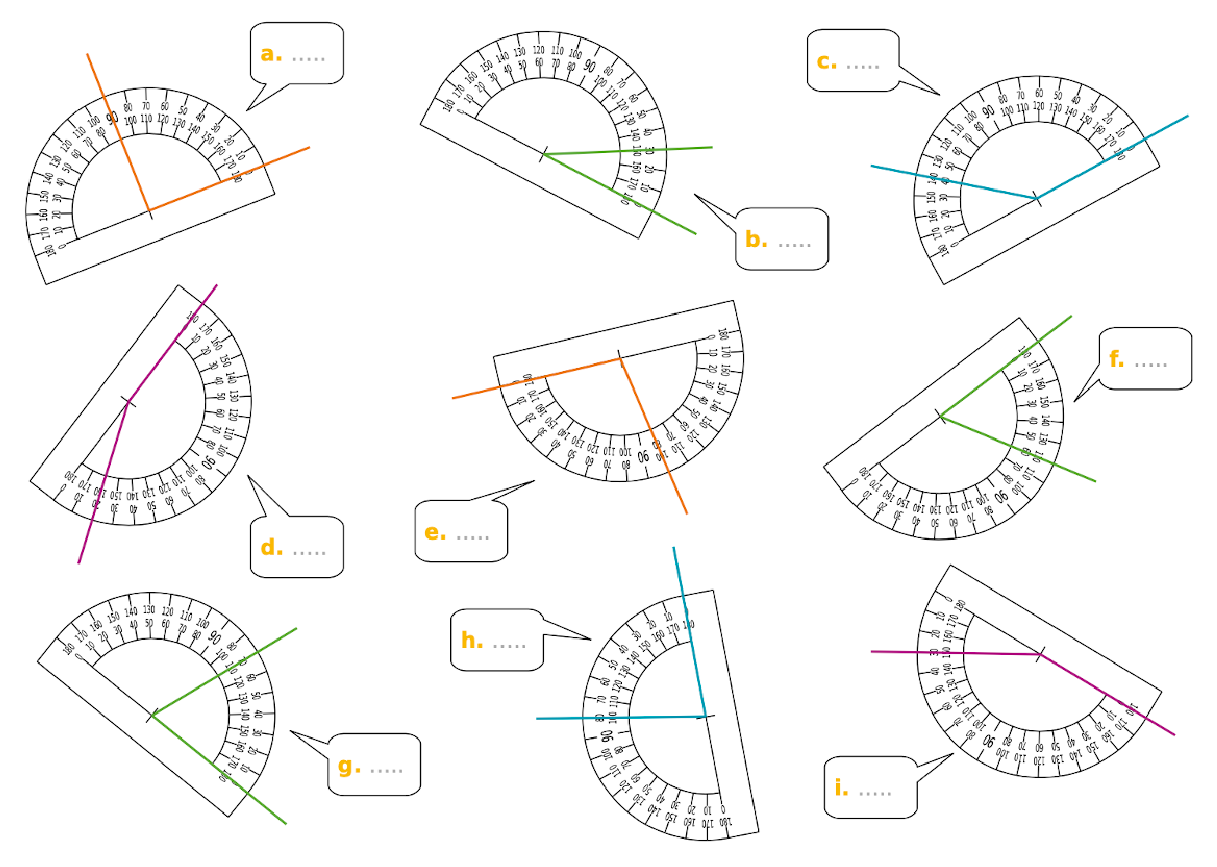
\includegraphics[width=14cm]{rapporteur}
   \end{center}
\end{exercice}

\begin{exercice} %2
   Dans chaque cas, construire la demi-droite $[Oy)$ telle que l'angle $\widehat{xOy}$ ait la mesure indiquée.
   \begin{center}
      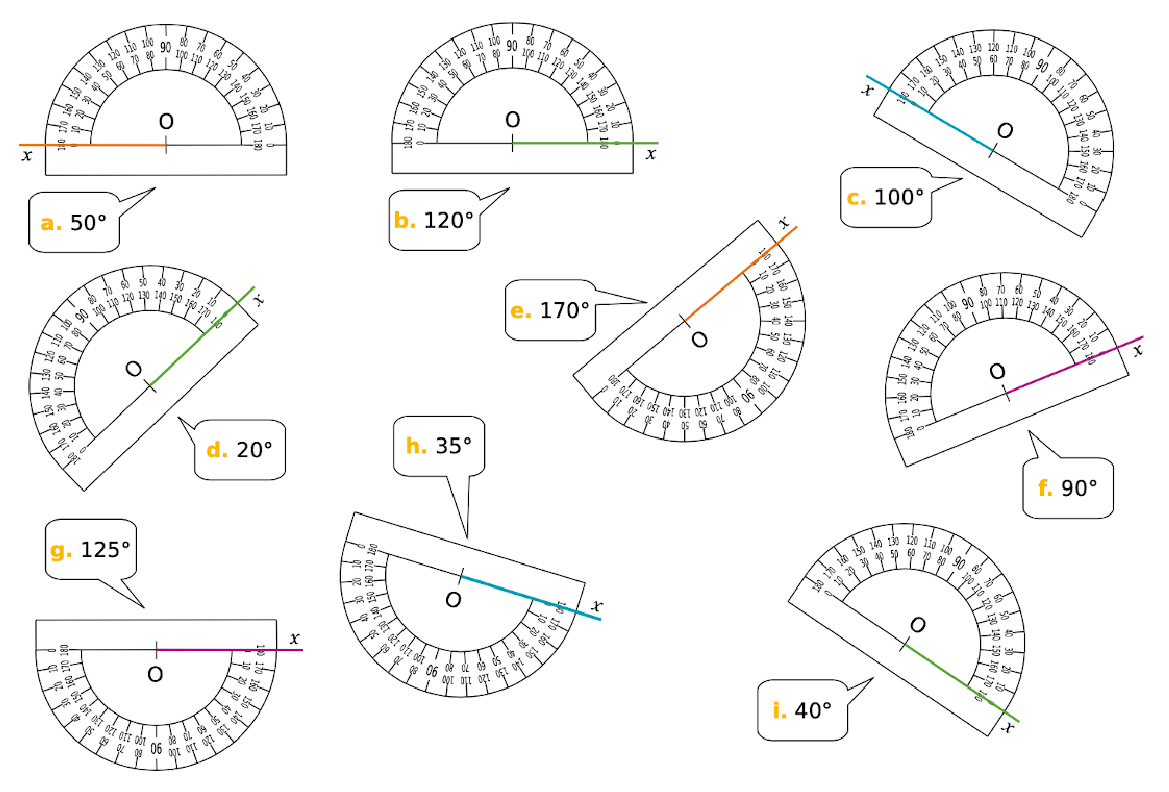
\includegraphics[width=14cm]{angle_rapporteur}
   \end{center}
\end{exercice}

\begin{exercice} %3

   Donner la mesure en degrés de chaque angle $\widehat{xOy}$.
   \begin{center}
      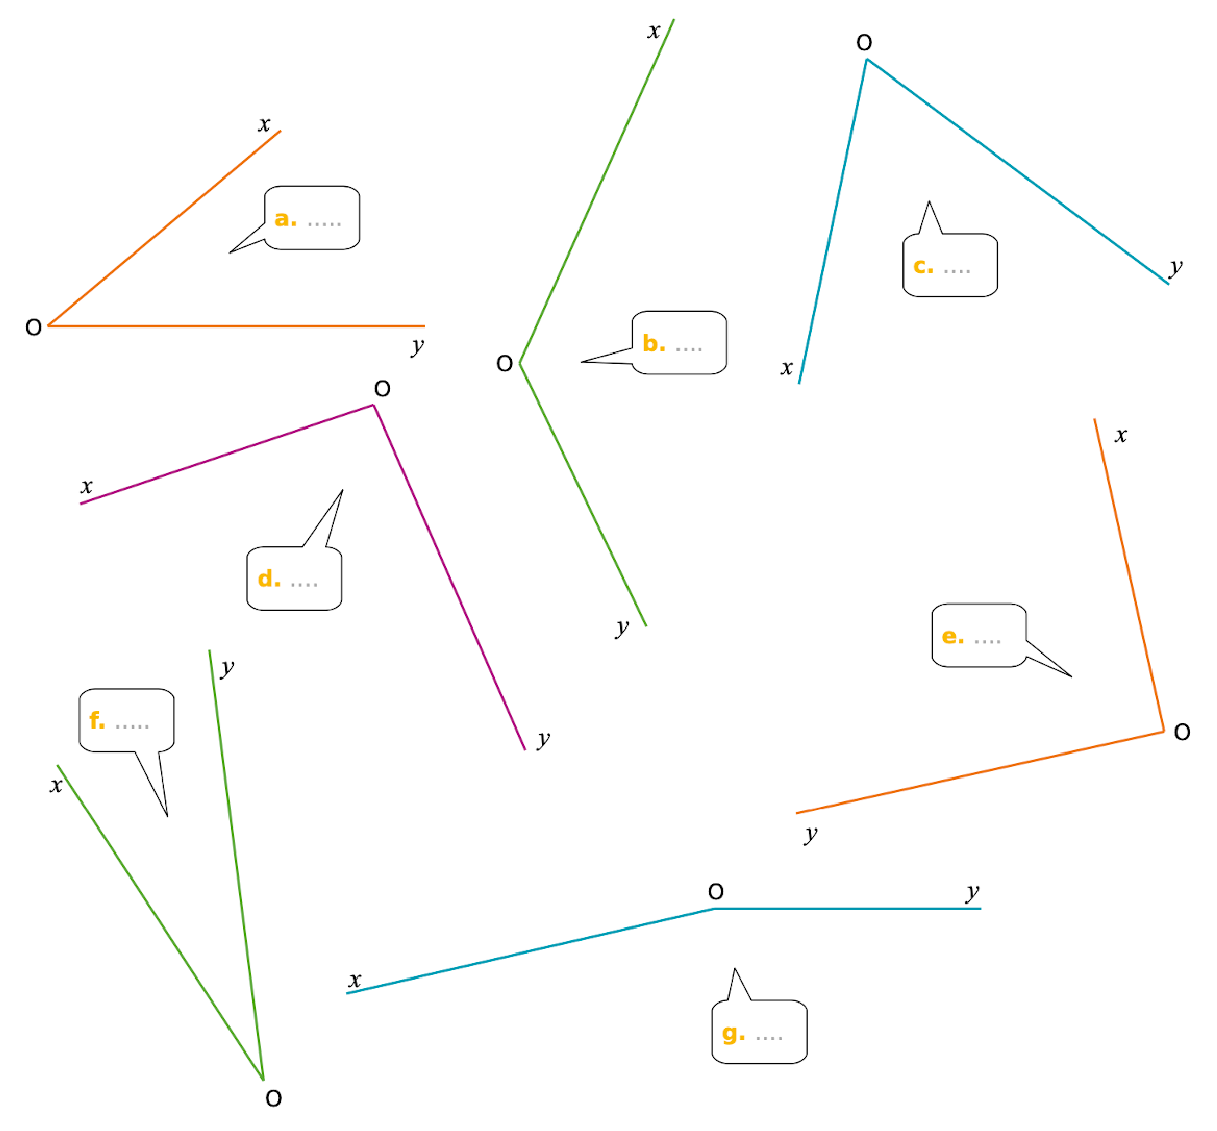
\includegraphics[width=16cm]{construire_angle}
   \end{center}
\end{exercice}

\begin{exercice} %4
   Reproduire la figure ci-contre en vraie grandeur.
   {\small
   \psset{unit=0.8}
   \begin{pspicture}(-1.5,2)(8,7)
      \pstGeonode[CurveType=polygon,PointSymbol=none,PosAngle={-40,45,90,180,220}](7,0.5){A}(7.5,5){B}(4,7){C}(0.5,4){D}(2,1){E}
      \pstGeonode[PointSymbol=none,PosAngle=-100](5,3){M}
      \pstLineAB{M}{A}
      \pstLineAB{M}{B}
      \pstLineAB{M}{C}
      \pstLineAB{M}{D}
      \pstLineAB{M}{E}
      \pstMarkAngle{M}{B}{A}{55\degre}
      \pstMarkAngle{A}{M}{B}{78\degre}
      \pstMarkAngle{B}{M}{C}{75\degre}
      \pstMarkAngle{D}{M}{E}{40\degre}
      \rput{40}(2,5.8){6 cm}
      \rput{283}(4.8,5.1){4 cm}
      \rput{-12}(2.9,3.8){6,5 cm}
      \rput{35}(3.2,2.2){5 cm}
      \rput{39}(6.2,4.35){4 cm}
   \end{pspicture}}
\end{exercice}

\vfill\hfill{\it\footnotesize Source : Les cahiers Sesamath 6\up{e}. Magnard-Sésamath 2017.}

%%%%%%%%%%%%%%%%%%%%%
%%%%%%%%%%%%%%%%%%%%%
\Recreation

\enigme[Coupe des quatre maisons de Poudlard]
   On a retrouvé dans un grimoire les points obtenus lors de la coupe des quatre maisons de Poudlard, par trimestre, et on souhaiterait obtenir un diagramme circulaire de chacun de ces résultats afin de mieux pouvoir les comparer.
   \partie[1\up{er} trimestre]
      \begin{minipage}{11cm}
         Voilà les points obtenus au premier trimestre par les différentes maisons :
         \begin{center}
            {\hautab{1.2}
            \small
            \begin{ltableau}{0.85\linewidth}{5}
               \hline
               Griffondor & Poufsouffle & Serdaigle & Serpentard & Total\\
               \hline
               100 & 90 & 120 & 50 & \\
               \hline
               & & & & \udeg{360} \\
               \hline
            \end{ltableau}}
         \end{center}
         \begin{enumerate}
            \item Compléter le tableau avec le total des points de l'ensemble des maisons.
            \item En déduire l'angle en degrés de chaque secteur pour chaque maison.
            \item Représenter les résultats dans le diagramme circulaire ci-contre.
         \end{enumerate}
      \end{minipage}
      \qquad
      \begin{minipage}{4cm}
         \begin{pspicture}(-2.8,-2.3)(2.3,2.3)
            \pscircle(0,0){2.3}
         \end{pspicture}
      \end{minipage}
      
   \partie[2\up{e} trimestre]
      \begin{minipage}{11cm}
         Voilà les points obtenus au deuxième trimestre par les différentes maisons :
         \begin{center}
            {\hautab{1.2}
            \small
            \begin{ltableau}{0.85\linewidth}{5}
               \hline
               Griffondor & Poufsouffle & Serdaigle & Serpentard & Total\\
               \hline
               60 & 50 & 20 & 50 & \\
               \hline
               & & & & \udeg{360} \\
               \hline
            \end{ltableau}}
         \end{center}
         \begin{enumerate}
            \item Compléter le tableau avec le total des points de l'ensemble des maisons.
            \item En déduire l'angle en degrés de chaque secteur pour chaque maison.
            \item Représenter les résultats dans le diagramme circulaire ci-contre.
         \end{enumerate}
      \end{minipage}
      \qquad
      \begin{minipage}{4cm}
         \begin{pspicture}(-2.8,-2.3)(2.3,2.3)
            \pscircle(0,0){2.3}
         \end{pspicture}
      \end{minipage}
            
   \partie[3\up{e} trimestre]
      \begin{minipage}{11cm}
         Voilà les points obtenus au troisième trimestre par les différentes maisons :
         \begin{center}
            {\hautab{1.2}
            \small
            \begin{ltableau}{0.85\linewidth}{5}
               \hline
               Griffondor & Poufsouffle & Serdaigle & Serpentard & Total\\
               \hline
               40 & 70 & 50 & 100 & \\
               \hline
               & & & & \udeg{360} \\
               \hline
            \end{ltableau}}
         \end{center}
         \begin{enumerate}
            \item Compléter le tableau avec le total des points de l'ensemble des maisons.
            \item En déduire l'angle en degrés de chaque secteur pour chaque maison.
            \item Représenter les résultats dans le diagramme circulaire ci-contre.
         \end{enumerate}
      \end{minipage}
      \qquad
      \begin{minipage}{4cm}
         \begin{pspicture}(-2.8,-2.3)(2.3,2.3)
            \pscircle(0,0){2.3}
         \end{pspicture}
      \end{minipage}
      
   \partie[total de l'année]
      \begin{minipage}{11cm}
         \begin{center}
            {\hautab{1.2}
            \small
            \begin{ltableau}{0.85\linewidth}{5}
               \hline
               Griffondor & Poufsouffle & Serdaigle & Serpentard & Total\\
               \hline
               & & & & \\
               \hline
               & & & & \udeg{360} \\
               \hline
            \end{ltableau}}
         \end{center}
         \begin{enumerate}
            \item Compléter le tableau avec le total des points sur l'année entière.
            \item En déduire l'angle en degrés de chaque secteur pour chaque maison.
            \item Représenter les résultats dans le diagramme circulaire ci-contre.
         \end{enumerate}
      \end{minipage}
      \qquad
      \begin{minipage}{4cm}
         \begin{pspicture}(-2.8,-2.5)(2.3,2.3)
            \pscircle(0,0){2.3}
         \end{pspicture}
      \end{minipage}


